\chapter{Epipolar Geometry and Fundamental Matrix}

\noindent
En la geometría de una única vista, la proyección de un punto tridimensional del espacio sobre el plano de la imagen introduce una pérdida irreversible de dimensionalidad. Dado un único punto proyectado $\mathbf{x}$, solo es posible realizar una retroproyección en el espacio en forma de rayo infinito sobre el cual descansa el punto 3D real. \\

\noindent
La \textbf{Geometría de Dos Vistas (Two-View Geometry)} resuelve esta ambigüedad introduciendo una segunda cámara posicionada en una ubicación arbitraria del espacio. El objetivo central de esta rama es modelar la relación geométrica intrínseca entre un punto 3D del espacio, su proyección en la primera imagen y su proyección homóloga en la segunda captura.

\section{Epipolar Geometry}
La geometría epipolar describe la geometría proyectiva intrínseca entre dos vistas independientes de una misma escena estática. Depende exclusivamente de los parámetros internos de las cámaras y de su movimiento relativo (coplanares rígidos), siendo totalmente independiente de la estructura de la escena tridimensional vista.

\subsection{Elementos Fundamentales de la Anatomía Epipolar}
\noindent
Consideremos dos cámaras con centros ópticos (o centros de proyección) localizados en $\mathbf{O}$ y $\mathbf{O}'$, respectivamente:

\begin{itemize}
    \item \textbf{Línea de Base (Baseline):} Es el segmento de recta física en el espacio tridimensional que conecta de forma directa los dos centros de proyección de las cámaras ($\mathbf{O}$ y $\mathbf{O}'$).
    \item \textbf{Epipoles -- $\mathbf{e}, \mathbf{e}'$:} el epípolo es matemáticamente la proyección del centro óptico de una cámara sobre el plano de la imagen de la otra cámara. 
    \begin{itemize}
        \item El epípolo izquierdo $\mathbf{e}$ es la proyección de $\mathbf{O}'$ en la imagen izquierda.
        \item El epípolo derecho $\mathbf{e}'$ es la proyección de $\mathbf{O}$ en la imagen derecha.
        \item Alternativamente, se definen como los puntos de intersección de la línea de base con ambos planos de imagen.
    \end{itemize}
    \item \textbf{Epipolar Plane:} es el plano tridimensional único delimitado y definido por el punto del espacio real $\mathbf{P}$ y los dos centros ópticos de las cámaras ($\mathbf{O}, \mathbf{O}', \mathbf{P}$). Al rotar el punto $\mathbf{P}$ por el espacio, este plano pivota utilizando la línea de base como su eje central de bisagra.
    \item \textbf{Epipolar Lines -- $\mathbf{l}, \mathbf{l}'$:} son las líneas rectas resultantes de la intersección del plano epipolar con los planos de imagen de cada cámara. Toda línea epipolar en una imagen contiene obligatoriamente al epípolo de dicha vista.
\end{itemize}
Podemo ver una representación de estos elementos en la Figura \ref{fig:epipolar_anatomy}.

\begin{figure}
    \centering
    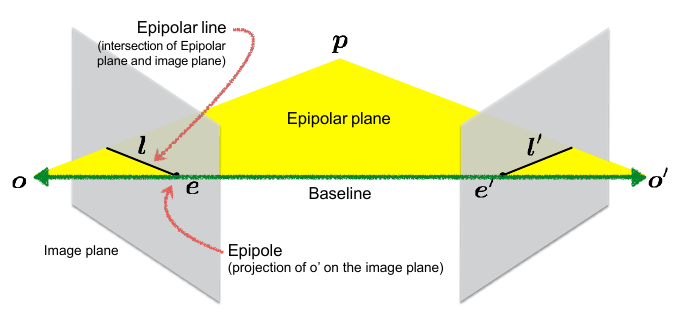
\includegraphics[width=0.8\textwidth]{img/epipolar_anatomy.png}
    \caption{Anatomía de la Geometría Epipolar: Línea de Base, Epípolos, Plano Epipolar y Líneas Epipolares}
    \label{fig:epipolar_anatomy}
\end{figure}

\subsection{Epipolar Constraint}
\noindent
El principio fundamental de la restricción epipolar dicta que:
\begin{quote}
    \textit{``Un punto geométrico medido en una primera imagen restringe la búsqueda de su correspondencia homóloga en la segunda vista a yacer estrictamente sobre la línea epipolar correspondiente.''} 
\end{quote}
\noindent
\textbf{Intuición Geométrica Crucial:} sin el uso de la restricción epipolar, encontrar el emparejamiento de un píxel requiere realizar una búsqueda bidimensional ($\mathcal{O}(N^2)$) por toda la superficie de la segunda imagen. Al aplicar este principio, el espacio de búsqueda \textbf{se colapsa de forma directa a una dimensión (1D)} a lo largo de la línea epipolar recta.

\subsection{Casos Especiales de Configuración de Cámaras}
\begin{enumerate}
    \item \textbf{Converging Cameras:} los epípolos son puntos finitos que se localizan frecuentemente dentro o cerca de los límites de la imagen, y las líneas epipolares convergen radialmente hacia ellos.
    \item \textbf{Parallel Cameras:} ocurre cuando los ejes de visión de ambas cámaras son estrictamente paralelos y perpendiculares a la línea de base. En este escenario geométrico, los centros ópticos proyectados se encuentran en el infinito proyectivo, lo que implica que \textbf{los epípolos divergen al infinito} ($\mathbf{e}, \mathbf{e}' \to \infty$). Consecuentemente, las líneas epipolares se vuelven paralelas entre sí y se alinean perfectamente de forma horizontal con las filas de los sensores píxel a píxel.
    \item \textbf{Forward Motion:} ocurre en trayectorias de traslación rectilínea a lo largo del eje óptico (ej. cámaras a bordo de vehículos). El epípolo coincide exactamente con el \textit{Foco de Expansión} (punto principal de la imagen), y las líneas epipolares divergen de forma radial desde dicho centro hacia afuera. 
    
    \begin{ejemplo}
        Imaginemos que vamos conduciendo por una autopista recta de noche. Si mirams al fondo, hay un punto exacto en el horizonte (el final de la carretera) del cual parecen nacer todas las líneas de los carriles y las farolas.
        \begin{itemize}
            \item \tbf{Físicamente}: ese punto del horizonte es el lugar hacia el que nos dirigimos.
            \item \tbf{En la imagen}: a ese punto de fuga se le llama \textit{Foco de Expansión}. Coincide de forma aproximada con el centro de tu imagen (el punto principal $(c_x, c_y)$ que estudiamos en la calibración).
        \end{itemize} 
    \end{ejemplo}
    
\end{enumerate}

\section{Matriz Esencial $\to$ Matriz Fundamental}

\subsection{La Matriz Esencial ($E$)}
\noindent
Propuesta por \tbf{Longuet-Higgins} en 1981, asume una configuración estéreo calibrada donde las matrices de parámetros intrínsecos de ambas cámaras actúan como matrices identidad ($K = K' = I$). En este espacio analítico, las coordenadas 2D de la imagen están expresadas directamente en el sistema de referencia métrico de la cámara. \\

\noindent
Imaginemos que estamos en un espacio tridimensional. Tenemos un punto físico en el mundo (por ejemplo, la esquina de una mesa) al que llamaremos $\mathbf{X}$ (en mayúscula para denotar que está en 3D). Para la cámara $1$, este punto se proyecta en la imagen como $\mathbf{x}$, y para la cámara $2$ se proyecta como $\mathbf{x}'$, dado por
\begin{equation*}
    \mathbf{x}' = R(\mathbf{x} - \mathbf{t})
\end{equation*}
donde para poder saber donde esta la cámara 2 con respecto a la cámara 1, se introduce una transformación rígida compuesta por una rotación $R$ y una traslación $\mathbf{t}$ que conecta ambos sistemas de referencia de las cámaras.\\

\noindent
Si nos paramos en el centro de la Cámara 1, podemos definir tres vectores que viven (están atrapados) dentro de ese mismo plano:
\begin{itemize}
    \item El vector $\mathbf{x}$ (que va del centro 1 al punto del objeto).
    \item El vector $\mathbf{t}$ (que va del centro 1 al centro 2).
    \item El vector $(\mathbf{x} - \mathbf{t})$ (que es el vector que va desde el centro 2 al punto del objeto, pero medido desde los ``ojos'' de la Cámara 1).
\end{itemize}
por lo que si tres vectores están en el mismo plano (son coplanares), significa que no tienen volumen en 3D. Podemos ver una represanticón de estos vectores en la Figura \ref{fig:epipolar_geometry}. El \tbf{scalar triple product} calcula el volumen del paralelepípedo que forman. Como están aplastados en un plano, ese volumen es cero:

$$(\mathbf{x} - \mathbf{t})^\top (\mathbf{t} \times \mathbf{x}) = 0$$
puesto que $x'=R(x-t)$, tenemos $(x-t)=R^{\top}x'$ (donde $R^{-1} = R^{\top}$ por ser matriz ortogonal), entonces

\begin{equation*}
    x'^{\top} R (t\times x) = 0
\end{equation*}
El \underline{truco maravilloso} de Longuet-Higgins, fue usar que the cross product $t \times x$ can be written as a matrix-vector multiplication using the skew-symmetric matrix $[t]_\times$:
\begin{equation*}
    t\times x=[t]_\times x \quad \text{ donde } [t]_\times = \begin{bmatrix}
     0 & -t_3 & t_2 \\
     t_3 & 0 & -t_1 \\
     -t_2 & t_1 & 0
    \end{bmatrix}
\end{equation*}
sabiendo que
\begin{equation*}
    t\times x = \det \begin{pmatrix} \hat{i} & \hat{j} & \hat{k} \\ t_1 & t_2 & t_3 \\ x_1 & x_2 & x_3 \end{pmatrix}=\big( (t_2 x_3 - t_3 x_2), \; (t_3 x_1 - t_1 x_3), \; (t_1 x_2 - t_2 x_1) \big)
\end{equation*}
y sustituyendo esto en la ecuación anterior
\begin{equation*}
    x'^{\top} R [t]_\times x = 0 \implies E = R [t]_\times
\end{equation*}
donde tenemos la \tbf{Longest-Higgins equation} 
\begin{equation*}
    \boxed{x'^{\top} E x = 0} \quad \text{ where } E = R [t]_\times
\end{equation*}
donde $E$ es la \textbf{Matriz Esencial} que encapsula la relación epipolar entre las dos vistas calibradas. \\

\begin{figure}
    \centering
    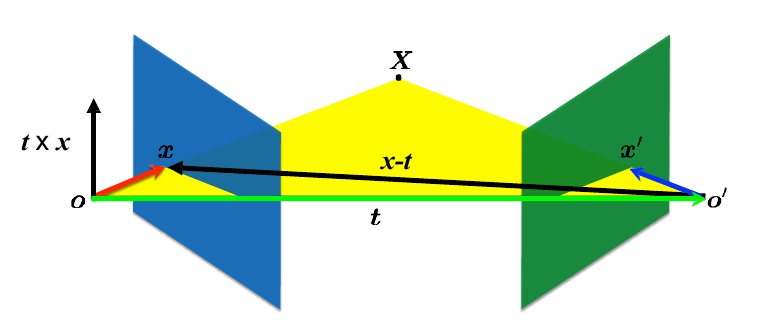
\includegraphics[width=0.8\textwidth]{img/epipolar_geometry.png}
    \caption{Vectores $\mathbf{x}$, $\mathbf{t}$ y $(\mathbf{x} - \mathbf{t})$ coplanares.}
    \label{fig:epipolar_geometry}
\end{figure}

\noindent
\tbf{Conclusión Conceptual de $E$}: la matriz esencial $E = R [\mathbf{t}]_\times$ codifica únicamente las propiedades extrínsecas de la escena (cómo está rotada una cámara respecto a otra y hacia dónde se ha desplazado). Su gran utilidad es que si un coche autónomo o un robot detecta un punto $\mathbf{x}$ en la primera cámara, al multiplicarlo por $E$ obtiene instantáneamente la línea exacta donde está obligado a buscar ese mismo punto en la segunda cámara.

\subsection{Fundamental Matrix ($F$)}
\noindent
Para modelar imágenes reales sin necesidad de calibración previa, eliminamos la suposición de matriz identidad parametrizando la transición desde las coordenadas métricas puras de la cámara ($\hat{\mathbf{x}}$) hacia las coordenadas reales de la pantalla medidas en píxeles normales ($\mathbf{x}$) mediante la inversa de los intrínsecos, es decir
\begin{equation}
    \hat{\mathbf{x}} = K^{-1}\mathbf{x} \quad \text{y} \quad \hat{\mathbf{x}}' = K'^{-1}\mathbf{x}' 
\end{equation}
recordemos que 
\begin{itemize}
    \item \tbf{$\hat{\mathbf{x}}$} es un vector en metros que te dice exactamente con qué inclinación entró el rayo de luz a la cámara, lo que viene a ser el rayo de luz de la cámara apuntando al espacio (2D homogéneo). Su tercera coordenada siempre vale 1 por diseño. No sabe a cuántos metros reales estaba el farol (perdió la profundidad), solo sabe en qué dirección venía el rayo.
    \item \tbf{$\mathbf{x}$} es el punto proyectado en coordenadas de píxeles de la imagen (en píxeles).
\end{itemize}
Sustituyendo estas expresiones en la matriz esencial, tenemos
\begin{equation}
    (K'^{-1}\mathbf{x}')^{\top} E (K^{-1}\mathbf{x}) = 0 \implies \mathbf{x}'^{\top} (K'^{-\top} E K^{-1}) \mathbf{x} = 0
\end{equation}
y definimos de este modo de forma única la \textbf{Matriz Fundamental ($F$)} con su ecuación correspondiente
\begin{equation}
    \boxed{x'^{\top} F x = 0} \quad \text{donde} \quad F = K'^{-\top} E K^{-1}
\end{equation}
Para diferenciar ambas matrices tenemos estas ideas cruciales:
\begin{itemize}
    \item La Matriz Esencial ($E$) solo entiende de geometría física en el mundo real (metros, ángulos, rotación, traslación). Requiere cámaras perfectamente calibradas.
    \item La Matriz Fundamental ($F$) entiende el lenguaje de la computadora (píxeles). Absorbe los parámetros intrínsecos de las cámaras y te permite relacionar dos imágenes directamente a partir de sus correspondencias de puntos sin saber qué cámara tomó la foto.
\end{itemize}


\subsection{Propiedades Matemáticas y Relaciones Algebraicas de $F$}
\begin{itemize}
    \item \textbf{Mapeo de Punto a Línea:} Multiplicar la matriz $F$ por las coordenadas homogéneas de un punto de la primera imagen computa de forma directa los coeficientes de la línea epipolar recta en la vista opuesta:
    \begin{align*}
        \mathbf{l}' &= F\mathbf{x} \quad (\text{Línea epipolar en la imagen derecha}) \\
        \mathbf{l} &= F^{\top}\mathbf{x}' \quad (\text{Línea epipolar en la imagen izquierda}) 
    \end{align*}

    \item \textbf{Grados de Libertad (DoF):} $F$ es una matriz cuadrada de tamaño $3 \times 3$. Al operar sobre un espacio homogéneo, está definida únicamente salvo un factor de escala multiplicativo global arbitrario (reduciendo sus parámetros libres de 9 a 8). Adicionalmente, al estar forzada analíticamente por la restricción de rango, pierde un grado de libertad extra, resultando en un total de \textbf{7 Grados de Libertad independientes}.
    \item \textbf{Restricción de Rango (Rank Constraint):} Debido a que la matriz antisimétrica $[\mathbf{t}]_{\times}$ posee intrínsecamente rango igual a 2 y las matrices de calibración e intrínsecos $K$ poseen rango completo ($3$), la multiplicación matemática dicta de forma estricta que la Matriz Fundamental posee una deficiencia de rango obligatoria:
    \begin{equation*}
        \text{Rank}(F) = 2 \implies \det(F) = 0 
    \end{equation*}
    \item \textbf{Relaciones Matemáticas con los Epípolos ($e, e'$):} Dado que todos los rayos de proyección convergen en los epípolos correspondientes, estos constituyen los vectores del espacio nulo analítico (\textit{Null Space}) derecho e izquierdo de la matriz $F$, respectivamente:
    \begin{align*}
        \boxed{F \mathbf{e} = 0} \quad &\implies \text{\textbf{e} vive en el espacio nulo derecho de $F$} \\
        \boxed{F^{\top} \mathbf{e}' = 0} \quad &\implies \text{\textbf{e}' vive en el espacio nulo izquierdo de $F$} 
    \end{align*}
    Podemos ver más claramente porque los epípolos pertenecen siempre a las líneas epipolares en la imagen para cada punto $\mathbf{x}$ en la Figura \ref{fig:epipolar_lines}. \\
    \noindent
    El resultado de la propiedad viene porque dada la primera propiedad se tiene $F \mathbf{x} = \mathbf{l}'$, y como $\mathbf{e}'$ pertenece a la línea epipolar $\mathbf{l}'$, entonces
    $$\mathbf{e}'^{\top} \mathbf{l}' = 0 \implies \mathbf{e}'^{\top} (F\mathbf{x}) = 0 \implies (\mathbf{e}'^{\top} F) \mathbf{x} = 0$$
    como vale para cualquier $\mathbf{x}$, entonces
    $$\mathbf{e}'^{\top} F = 0 \implies F^{\top} \mathbf{e}' = 0$$
    \begin{figure}
        \centering
        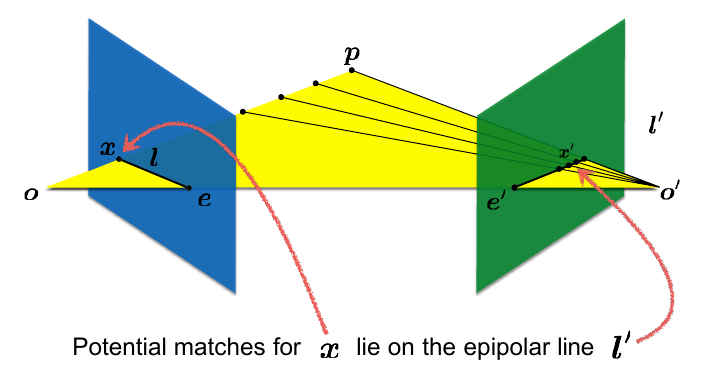
\includegraphics[width=0.8\textwidth]{img/epipolar_lines.png}
        \caption{El mapeo de un punto $\mathbf{x}$ a su línea epipolar $\mathbf{l}'$ en la imagen derecha mediante la multiplicación por $F$.}
        \label{fig:epipolar_lines}
    \end{figure}
\end{itemize}

\section{Estimación de la Matriz Fundamental ($F$)}

\subsection{Eight-Point Algorithm}
\noindent
Cada pareja de puntos correspondientes conocidos $\{\mathbf{x}_m, \mathbf{x}'_m\}$ en coordenadas homogéneas de píxeles $\mathbf{x}_m = [x_m, y_m, 1]^{\top}$ y $\mathbf{x}'_m = [x'_m, y'_m, 1]^{\top}$ debe satisfacer de forma estricta la ecuación epipolar:

\begin{equation*}
    \begin{bmatrix} x'_m & y'_m & 1 \end{bmatrix} 
    \begin{bmatrix} f_1 & f_2 & f_3 \\ f_4 & f_5 & f_6 \\ f_7 & f_8 & f_9 \end{bmatrix}
    \begin{bmatrix} x_m \\ y_m \\ 1 \end{bmatrix} = 0 
\end{equation*}
Al expandir algebraicamente la multiplicación término a término, se demuestra de forma analítica que \textbf{un único emparejamiento de puntos aporta exactamente una única ecuación lineal limpia} con 9 incógnitas:
\begin{equation*}
    x_m x'_m f_1 + y_m x'_m f_2 + x'_m f_3 + x_m y'_m f_4 + y_m y'_m f_5 + y'_m f_6 + x_m f_7 + y_m f_8 + f_9 = 0
\end{equation*}
Al recolectar e indexar un conjunto mínimo de $M \ge 8$ correspondencias puntuales discretas, podemos apilar las filas de coeficientes numéricos medidos para construir un sistema homogéneo lineal matricial de la forma:
\begin{equation*}
    A \mathbf{f} = \mathbf{0} 
\end{equation*}
donde $A$ es una matriz gigante de tamaño $M \times 9$, y $\mathbf{f} = [f_1, f_2, \dots, f_9]^{\top}$ corresponde al vector largo vectorizado que almacena las incógnitas de la cámara.

\subsubsection{Resolución Matemática mediante Descomposición SVD}
\noindent
Para evitar el colapso del sistema matemático hacia la solución trivial obvia ($\mathbf{f} = \mathbf{0}$), se formula el problema bajo la teoría de Mínimos Cuadrados Totales (\textit{Total Least Squares}) imponiendo una Restricción de Norma Unidad para la escala:
\begin{equation*}
    \min_{\mathbf{f}} \|A \mathbf{f}\|^2 \quad \text{sujeto a} \quad \|\mathbf{f}\|^2 = 1 
\end{equation*}
El teorema del álgebra lineal demuestra que la solución óptima a esta minimización estructurada se obtiene de forma directa calculando la \textbf{Descomposición en Valores Singulares (SVD)} de la matriz de coeficientes del sistema $A$:
\begin{equation*}
    A = U \Sigma V^{\top} 
\end{equation*}
El vector de incógnitas óptimo $\mathbf{f}$ se extrae tomando de forma directa \textbf{la última columna de la matriz $V$} (el autovector correspondiente al menor valor singular de la matriz). Posteriormente, se realiza una operación de cambio de forma (\textit{reshape}) de $9 \times 1$ a una rejilla de $3 \times 3$ para moldear la matriz estimadora inicial $F$.

\subsection{El Defecto del Algoritmo de 8 Puntos Estándar y Necesidad de Normalización}
\noindent
En imágenes digitales reales (ej. resolución Full HD $1920 \times 1080$), las coordenadas en píxeles de los extremos superiores de la matriz $A$ son del orden de $10^3$, lo que provoca que términos cuadráticos cruzados como $x_m x'_m$ alcancen magnitudes del orden de $10^6$. En contraste, las últimas columnas de la matriz $A$ contienen coordenadas constantes iguales a $1$ ($10^0$), que se ve tan fácilmente sabiendo que 
$$A_m = \begin{bmatrix} x x' & x y' & x & y x' & y y' & y & x' & y' & 1 \end{bmatrix}$$
donde $x_m = [x, y, 1]^\top$ (en la primera imagen) y $x'_m = [x', y', 1]^\top$ (en la segunda imagen). \\

\noindent
Esta enorme \textbf{disparidad de órdenes de magnitud} causa que la matriz de datos $A$ posea un número de condición pésimo y esté extremadamente mal condicionada numéricamente. Cualquier leve ruido de medición de SIFT en los píxeles desviará catastróficamente el cálculo de mínimos cuadrados.

\observacion{
    Aqui se nombra el algoritmo SIFT, puesto que las parejas que usaremos para construir la matriz $A$ las extraemos de los descriptores SIFT, que aunque son robustos, no son perfectos y contienen un porcentaje de correspondencias erróneas (outliers) que también afectan a la calidad de la estimación de $F$. Esto último lo solucionaremos usando RANSAC (se explica más adelante).
}
\subsection{El Algoritmo de los 8 Puntos Normalizado de Hartley}
\noindent
Para solventar el mal condicionamiento numérico, Richard Hartley propuso en 1995 un pipeline de precondicionamiento obligatorio estructurado en los siguientes pasos secuenciales:

\begin{enumerate}
    \item \textbf{Normalización de Coordenadas:} Antes de construir la matriz $A$, se calculan de forma independiente dos matrices de transformación afín $T$ y $T'$ para la imagen izquierda y derecha, respectivamente. Estas transformaciones aplican un cambio de escala y traslación sobre los puntos de modo que cumplan dos condiciones estadísticas:
    \begin{itemize}
        \item El centroide de masa (media geométrica) de todos los puntos de la imagen se desplaza de forma exacta hacia el origen de coordenadas cartesianas $(0,0)$.
        \item Los vectores de píxeles se escalan de forma homogénea para que la distancia media cuadrática desde el origen de coordenadas recalculado hacia los puntos normalizados sea exactamente igual a $\sqrt{2}$ píxeles (logrando que el rango promedio de los datos oscile estrictamente en el intervalo $[-1, 1]$).
    \end{itemize}
    Los nuevos puntos normalizados se computan como $\tilde{\mathbf{x}}_m = T \mathbf{x}_m$ y $\tilde{\mathbf{x}}'_m = T' \mathbf{x}'_m$.
    
    \item \textbf{Estimación Lineal:} Se construye la matriz del sistema utilizando los puntos normalizados $\{\tilde{\mathbf{x}}_m, \tilde{\mathbf{x}}'_m\}$, se calcula su SVD y se extrae la matriz fundamental normalizada intermedia, denotada como $\tilde{F}$.
    
    \item \textbf{Imposición de la Restricción de Rango 2 (Rank Enforcing):} La matriz numérica calculada $\tilde{F}$ en el paso anterior no poseerá rango igual a 2 de forma perfecta debido al ruido analítico presente en las mediciones ($\det(\tilde{F}) \neq 0$). Para forzar la consistencia epipolar, calculamos su SVD interna:
    \begin{equation*}
        \tilde{F} = U \Sigma V^{\top} = U \begin{bmatrix} \sigma_1 & 0 & 0 \\ 0 & \sigma_2 & 0 \\ 0 & 0 & \sigma_3 \end{bmatrix} V^{\top}
    \end{equation*}
    Donde los valores singulares están ordenados en orden descendente ($\sigma_1 \ge \sigma_2 \ge \sigma_3$). Se aplica el teorema de Eckart-Young eliminando el menor valor singular de la diagonal (forzando $\sigma_3 = 0$) para construir una nueva matriz diagonal corregida $\Sigma'$:
    \begin{equation*}
        \Sigma' = \begin{bmatrix} \sigma_1 & 0 & 0 \\ 0 & \sigma_2 & 0 \\ 0 & 0 & 0 \end{bmatrix} 
    \end{equation*}
    Se reconstruye la matriz fundamental normalizada de rango corregido mediante la multiplicación:
    \begin{equation*}
        \tilde{F}_{\text{coaccionada}} = U \Sigma' V^{\top}
    \end{equation*}
    
    \item \textbf{Des-normalización Final al Espacio de Unidades Original:} Para recuperar la matriz aplicable sobre las coordenadas de píxeles reales de la foto inicial, se deshace algebraicamente el precondicionamiento aplicando las transformaciones transpuestas inversas de Hartley:
    \begin{equation*}
        \boxed{F = T'^{\top} \tilde{F}_{\text{coaccionada}} T}
    \end{equation*}
\end{enumerate}

\subsection{Uso de RANSAC en la Estimación Práctica}
\noindent
En entornos prácticos y reales de ingeniería, las correspondencias extraídas mediante descriptores como SIFT contienen un porcentaje elevado de emparejamientos erróneos (llamados analíticamente \textit{outliers}) debido a texturas repetitivas o cambios bruscos de iluminación. \\ 

\noindent
Dado que el criterio de mínimos cuadrados del algoritmo SVD es extremadamente sensible a datos erróneos, se integra de forma mandatoria el algoritmo robusto \textbf{RANSAC (Random Sample Consensus)}. RANSAC toma repetidamente subconjuntos aleatorios de solo 8 parejas de puntos, estima una matriz candidata $F$, y cuenta cuántos puntos del conjunto global la validan actuando como \textit{inliers}. Al finalizar las iteraciones, se descartan los \textit{outliers} y se calcula la matriz fundamental definitiva mediante el algoritmo normalizado utilizando únicamente el conjunto purificado de correspondencias correctas.
